\documentclass{article}

\usepackage[a4paper, total={6.5in, 11in}]{geometry}
\usepackage{amsmath}
\usepackage[dvipsnames]{xcolor}
\usepackage{graphicx}
\graphicspath{{titech/CSC.T438.DistributedAlgorithms/HW2/}}
%\usepackage{wrapfig}

\begin{document}

\section{Navigation: Raymond}

\subsection{Complement the request queues at each process for the situation where the object takes the longest possible time to return back to $p_6$.}

%\begin{wrapfigure}{r}{0.25\textwidth} %this figure will be at the right
%    \centering
%    \includegraphics[width=0.25\textwidth]{img}
%\end{wrapfigure}

\begin{minipage}{.45\textwidth}
  \begin{itemize}
    \item $p_1: p_1$
    \item $p_2: p_1, p_3, p_2$
    \item $p_3: p_3$
    \item $p_4: p_2, p_7, p_4$
    \item $p_5: p_5$
    \item $p_6: p_4, p_6$
    \item $p_7: p_5, p_8, p_7$
    \item $p_8: p_8$
  \end{itemize}
\end{minipage}
\begin{minipage}{.45\textwidth}
  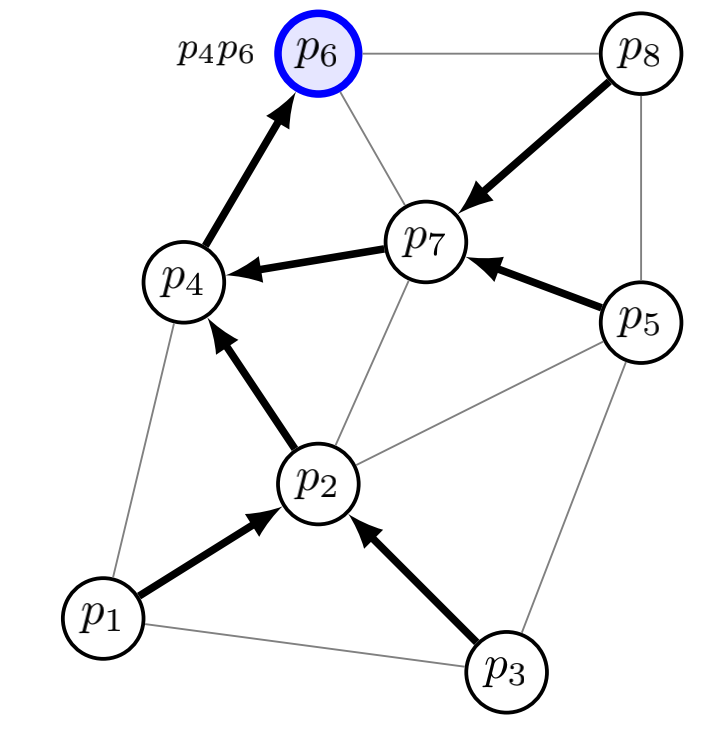
\includegraphics[width=\textwidth]{p1}
\end{minipage}

Object returns to $p_6$ after 14 steps.\\

Actually, whether $p_2,p_4,and\;p_7$ issue request or not will not affect the number of steps, because they will use the object in place without any extra steps. And it's meaningless in this situation, because every process only sends the request once, there is no different between once and multiple times.

\subsection{Express the path that the object follows after being released as a sequence of process identities.}
\textcolor{black}{$p_6$},\textcolor{black}{$p_4$},\textcolor{black}{$p_2$},\textcolor{red}{$p_1$},\textcolor{black}{$p_2$},\textcolor{red}{$p_3$},\textcolor{red}{$p_2$},\textcolor{black}{$p_4$},\textcolor{black}{$p_7$},\textcolor{red}{$p_5$},\textcolor{black}{$p_7$},\textcolor{red}{$p_8$},\textcolor{red}{$p_7$},\textcolor{red}{$p_4$},\textcolor{red}{$p_6$}

\subsection{Prove the absence of starvation.}
Assume that the object is located at $p_j$ and $p_i$ sent REQUEST(i) to its parent $p_{parent_i}$. $p_{parent_i}$ either already sent REQUEST($parent_i$) when the queue is not empty or sent REQUEST($parent_i$) immediately when the queue is empty. And $parent_i$'s paret will do the same thing, etc. For convenience, assume that $p_k$ is the root of the subtree which $p_i$ belongs to. Due to the spanning tree, the REQUEST(k) will arrive the root where the object is located at $p_j$. At that time, if $p_j$ is interested in the object, it will enqueue the REQUEST(k). After $p_j$ releases the object, it will send the object to the head of the queue. If $p_k$ is the head, everything goes well. Otherwise,  the object will be sent to another process with a new REQUEST(j) which means the object will go back to $p_j$ and will send the object to $p_k$ eventually. Actually every process will do the same thing as $p_j$ when it get the object, so every process in the queue will get the object. So $p_i$ eventually obtains the object.\\
On the other hand, every process uses the FIFO queue to buffer the request, so the process will send the object to all requests in order. Furthermore, the process will suppress an element in the queue when sending the object. Assume that REQUEST(i) is the k-th element in the $p_j$'s queue, $p_j$ will send the object to the $p_i$ at the certain k-th time.\\
Q.E.D.

\section{Mutual Exclusion: Arbitrary Graph}
Assume that the permission set is all the processes. \\
\begin{enumerate}
  \item Using the PIF to construct the spanning tree. \\
  \item Initialize the permission on one process arbitrarily. \\
  \item Using Raymond's algorithm to deliver the permission in order to mutual exclusion.
\end{enumerate}

\section{Ricart-Agrawala}
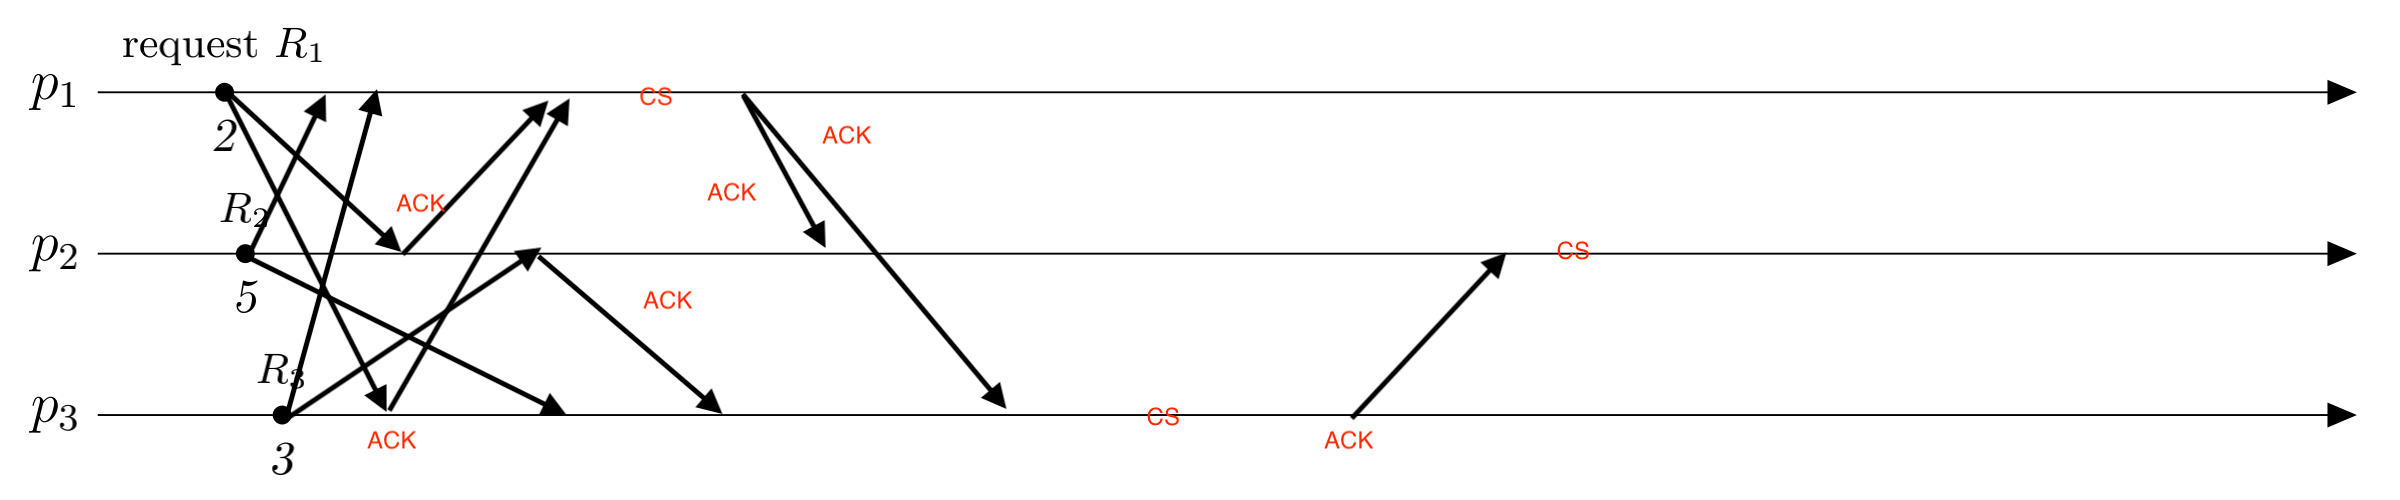
\includegraphics[width=\textwidth]{p3}

\section{Chandy-Misra}
Initialization
\begin{enumerate}
  \item $cs\_state_i = out$ \\
  \item $perm\_delayed_i = \emptyset$ \\
  \item $PERMISION({i, j})$ is at $p_i$ \\
  \item $perm\_state_i[j] = used$ \\
\end{enumerate}


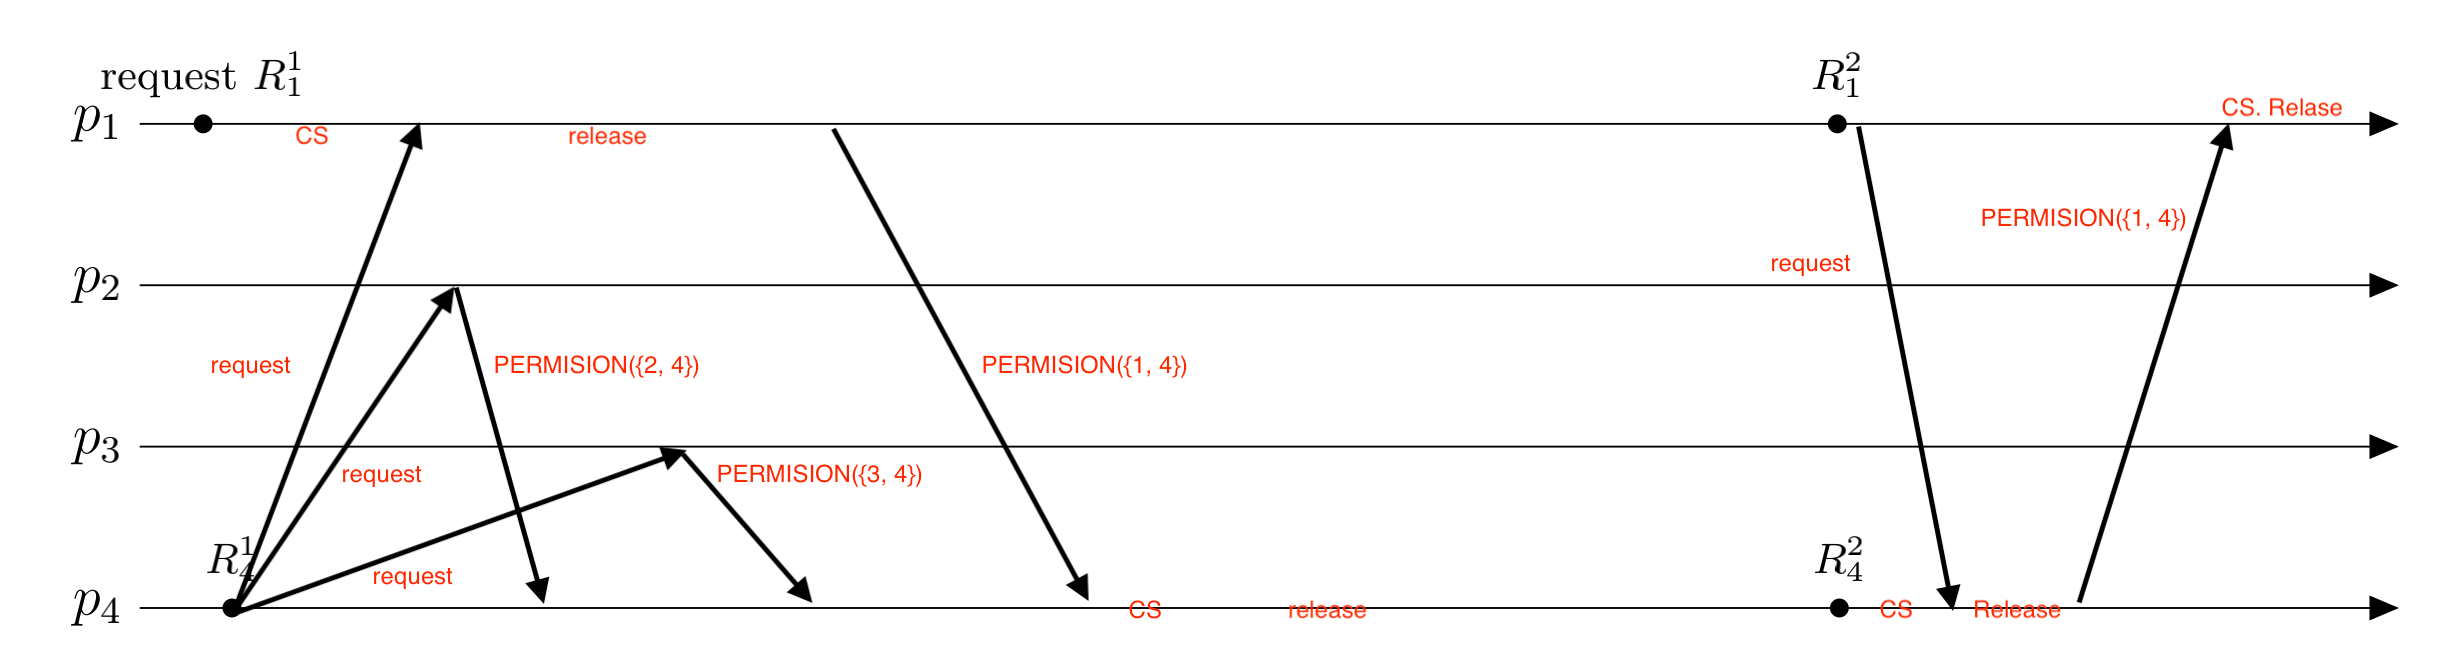
\includegraphics[width=\textwidth]{p4}


\section{Quorum}
\begin{itemize}
  \item $R_1: p_1,p_2,p_3,p_4$ \\
  \item $R_2: p_2,p_5,p_6,p_7$ \\
  \item $R_3: p_3,p_6,p_8,p_9$ \\
  \item $R_4: p_4,p_7,p_9,p_{10}$ \\
  \end{itemize}



\end{document}
